\documentclass{article}
% Preamable
\usepackage[margin=1in,headheight=12pt,includehead,includefoot]{geometry}
\usepackage{fancyhdr}
\usepackage{amsmath}
\usepackage{amssymb}
\usepackage{pifont} %For checkmark symbol in itemizing
\renewcommand{\labelitemii}{\ding{51}} %Change the item label level2
\usepackage{epsfig} %For including EPS graphic files
\usepackage{natbib} %For bibliography citation command
\usepackage{hologo} %For BibTeX logo
\usepackage{subfigure} %For making subfigure
\usepackage{pdfsync} %For skim
\usepackage{siunitx}
%\usepackage{kotex}
\usepackage{tabularx}
\usepackage{caption}
\usepackage{booktabs}
\usepackage{ltablex,booktabs}
\usepackage{threeparttable}
\usepackage{amsthm}

% Line break at ',','.','/','[' for texttt
\renewcommand{\texttt}[1]{%
  \begingroup
  \ttfamily
  \begingroup\lccode`~=`/\lowercase{\endgroup\def~}{/\discretionary{}{}{}}%
  \begingroup\lccode`~=`[\lowercase{\endgroup\def~}{[\discretionary{}{}{}}%
  \begingroup\lccode`~=`.\lowercase{\endgroup\def~}{.\discretionary{}{}{}}%
  \begingroup\lccode`~=`,\lowercase{\endgroup\def~}{,\discretionary{}{}{}}%
  \catcode`/=\active\catcode`[=\active\catcode`.=\active\catcode`,=\active
  \scantokens{#1\noexpand}%
  \endgroup
}

% Include figure path
\graphicspath{{./figures/}}

% Macro
% log 180826
\newcommand{\bi}{\begin{itemize}}
\newcommand{\ei}{\end{itemize}}




% Fancy header
\pagestyle{fancy}
\fancyhead{} %clear all header fields
\rhead{\bf Weekly progress report (\today)}
\lfoot{From: JhY}
\cfoot{To: JwN}
\rfoot{\thepage}
\renewcommand{\headrulewidth}{0.4pt} %use renewcommand to change the default settings
\renewcommand{\footrulewidth}{0.4pt}

% Title; this section will be printed in a titlepage by \maketitle command
\title{Weekly Progress Report}
\author{Jihwan Yoon}
\date{\today}

% Begin document
\begin{document}

% Default setting
\begin{center}
 {\LARGE \bf Weekly Progress Report}\\[15pt]
 {\Large From : Jihwan Yoon\\[5pt]  To : Prof. Jaewook Nam\\[10pt] Date: \today}\\[30pt]
\end{center}


\section{Major Tasks}
\begin{enumerate}
 \item Reading the Research Papers (Semi Lee, Jaeki Lee, Gates).
       \begin{itemize}
        \item Reading Prof. Gates' thesis\cite{gates1999slot} and Semi Lee's thesis for Frequency Analysis.
        \item Reading the papers of Jaeki Lee\cite{lee2016simple} and Semi Lee\cite{lee2015analysis}.
       \end{itemize}
 \item FEniCS.
 \item Silver Nanowire Project.
       \begin{itemize}
        \item Integrating equations of analytic 1-D Visco-Capillary model by using Python.
       \end{itemize}
\end{enumerate}
\vspace{5mm}


\section{Works Completed}
\begin{enumerate}
\item Experiment note and KIMM ppt.
 \item 4-AP experiment with KA.
 \item Raman spectrum. Because the wavelength of the laser is 532 nm, it was impossible to measure the thin film.
 \item XPS(X-ray photo-electron spectroscopy) and SEM-EDS(Energy-dispersive spectrometry) are recommendable. 
\end{enumerate}


\vspace{5mm}

\section{Works in Progress}
\begin{enumerate}
\item FEM Study.

 \item Silver Nanowire Project.
       \begin{itemize}
        \item Reviewing the thesis of Prof. Gates\cite{gates1999slot}.
        \item Utilizing the dynamic contact angle of Cox\cite{cox1986dynamics}.
        \item Confinement makes me ask definition of DCA. Therefore, I am now following up the paper of O.K. and Wonki Ahn.
        \begin{figure}[!ht]
\centering
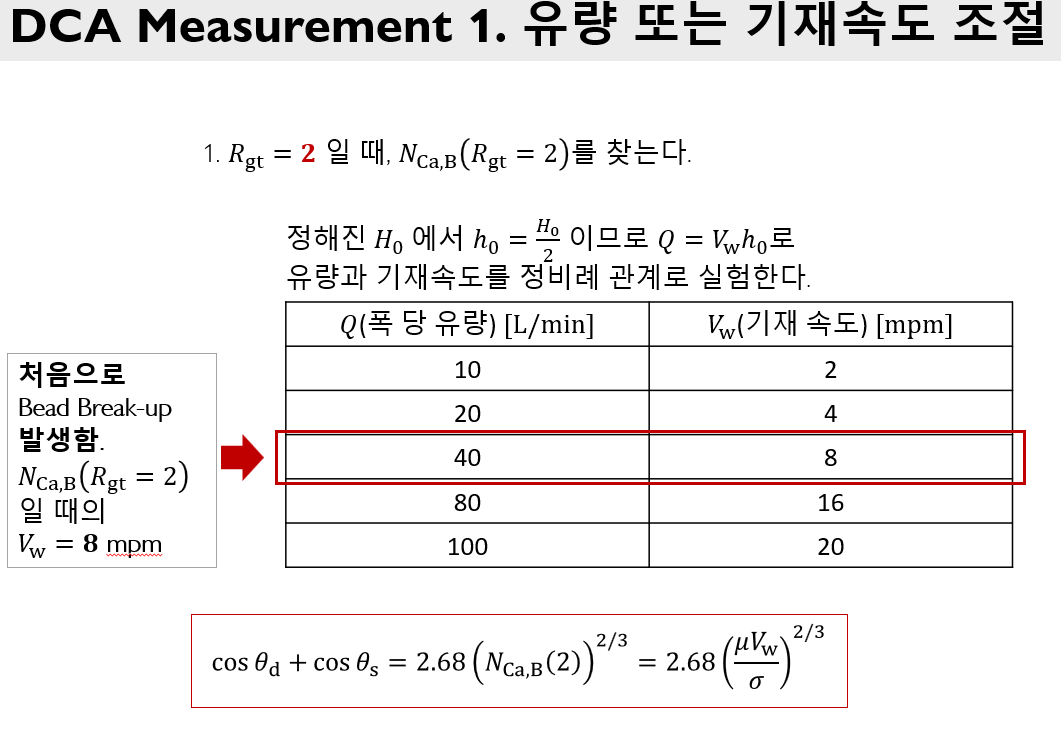
\includegraphics[scale=0.35]{figures/DCA_measurement_q_or_v.png}
\caption{DOF=1, MV=q or v}
\end{figure}
\item DCA in slot coating
\newline \newline
$ V_\textup{w}^{*} $ is the critical velocity when the Bead Break-up firstly appears at that configuration of die lip.\newline
$\theta_\textup{d}^{*} $ is the critical dynamic contact angle in a confined system(slot coating station) when the Bead Break-up firstly appears at that configuration of die lip.
$$ at\:  R_\textup{gt}=3 $$ : We can manipulate $H_0$. However, this equation is a simplified form and not accurate.
$$ \cos\theta_\textup{d}^{*} + \cos\theta_\textup{s}=6\left [ \frac{L_\textup{d}}{H_0}\left ( 1-\frac{2}{3} \right ) \right ]\frac{\mu V_\textup{w}^{*}}{\sigma}+1.34\cdot 3\cdot \left ( \frac{\mu V_\textup{w}^{*}}{\sigma} \right)^{2/3} $$
\newline
$$ at\:  R_\textup{gt}=2 $$ : We cannot manipulate anything. However, this equation is accurate because $ R_\textup{gt}=2 $ is a role of magic number in this physical system. This equation is the key of the idea of DCA in a slot coating process.
$$ \cos\theta_\textup{d}^{*} + \cos\theta_\textup{s}=1.34\cdot 2\cdot \left ( \frac{\mu V_\textup{w}^{*}}{\sigma} \right)^{2/3} $$
        
\end{itemize}

\end{enumerate}

\begin{table}
      \footnotesize
      \centering
      \begin{threeparttable}
      
      \caption{Caption of my Table}\label{tab:perflogcross}
      
      \begin{tabular}{
        l
        S[table-format=-1.3,table-figures-uncertainty=1]
        S[table-format=-1.3,table-figures-uncertainty=1]
        S[table-format=-1.3,table-figures-uncertainty=1]
        S[table-format=-1.3,table-figures-uncertainty=1]
      }
      \toprule
      & {Sensitivity} & {Specificity} & {BACC}& {Threshold} \\
      \midrule
      Full & 0.555 \pm 0.118 & 0.924 \pm 0.028 & 0.738 \pm 0.059 & 0.235 \pm 0.029 \\
      AIC  & 0.560 \pm 0.110 & 0.927 \pm 0.029 & 0.743 \pm 0.054 & 0.234 \pm 0.030 \\
      BIC  & 0.527 \pm 0.126 & 0.924 \pm 0.033 & 0.725 \pm 0.068 & 0.231 \pm 0.031 \\ 
      \bottomrule
      \end{tabular}
      \end{threeparttable}
\end{table}

%%%%%%%%%%%%%%%%%%%%%%%%%%%%%%%%%%%%%%%%%%%%%%%%%%%%%%%%%%%%%%%%%%%%%%
%                            References                              %
%%%%%%%%%%%%%%%%%%%%%%%%%%%%%%%%%%%%%%%%%%%%%%%%%%%%%%%%%%%%%%%%%%%%%%
\clearpage
\bibliographystyle{unsrt}
\bibliography{ref}
\end{document}
